\documentclass[aspectratio=169, 9pt]{beamer}

% Tema e colori
\usetheme{Madrid}
\usecolortheme{beaver}
\usepackage{graphicx}
\usepackage{amsmath}
\usepackage{booktabs}
\usepackage{multicol}
\usepackage{tikz}
\usepackage{fontawesome}

% Definizione della palette di colori (massimo 4 colori)
\definecolor{unibs}{HTML}{3D5895}
\definecolor{unibsLight}{HTML}{6D88B5}
\definecolor{unibsDark}{HTML}{1D3875}
\definecolor{accent}{HTML}{B87D3D}

% Personalizzazione
\setbeamercolor{structure}{fg=unibs}
\setbeamercolor{title}{fg=white, bg=unibs}
\setbeamercolor{frametitle}{fg=white, bg=unibs}
\setbeamercolor{block title}{bg=unibsLight!30, fg=unibsDark}
\setbeamercolor{block body}{bg=unibsLight!10}
\setbeamercolor{alerted text}{fg=accent}

% Miglioramento stile per punti elenco
\setbeamertemplate{itemize item}{\color{unibs}$\bullet$}
\setbeamertemplate{itemize subitem}{\color{unibsLight}$\circ$}

% Margini e dimensioni
\setbeamersize{text margin left=1.5cm}
\setbeamersize{text margin right=1.5cm}


% Rimuovere i pulsanti di navigazione
\beamertemplatenavigationsymbolsempty

% Imposta piè di pagina coerente
\setbeamertemplate{footline}{%
  \leavevmode%
  \hbox{%
    \begin{beamercolorbox}[wd=.15\paperwidth,ht=2.3ex,dp=1ex,left]{author in head/foot}%
      \usebeamerfont{author in head/foot}\hspace*{2ex}\insertshortauthor
    \end{beamercolorbox}%
    \begin{beamercolorbox}[wd=.70\paperwidth,ht=2.3ex,dp=1ex,center]{title in head/foot}%
      \usebeamerfont{title in head/foot}\insertshorttitle
    \end{beamercolorbox}%
    \begin{beamercolorbox}[wd=.15\paperwidth,ht=2.3ex,dp=1ex,right]{date in head/foot}%
      \usebeamerfont{date in head/foot}\insertshortdate{}\hspace*{2ex}
      \insertframenumber{} / \inserttotalframenumber\hspace*{2ex}
    \end{beamercolorbox}%
  }%
  \vskip0pt%
}

% Informazioni presentazione
\title{Sensibilità alle EMI di un amplificatore\\inverter based in tecnologia CMOS 180nm}
\author{Luca Brescia}
\institute{Università degli Studi di Brescia\\Dipartimento di Ingegneria dell'Informazione}
\date{\today}

\begin{document}

% Slide del titolo
\begin{frame}
    \titlepage
    \begin{center}
        \vspace{-1cm}
        
\includegraphics[height=1.2cm]{img/logo_unibs.pdf}
    \end{center}
\end{frame}

% Outline della presentazione
\begin{frame}{Contenuti}
    \tableofcontents
\end{frame}

\section{Introduzione}

% Introduzione alle EMI
\begin{frame}{Introduzione al problema delle EMI}
    \begin{columns}
        \column{0.6\textwidth}
        \textbf{Interferenze Elettromagnetiche (EMI):}
        \begin{itemize}
            \item Segnali indesiderati che compromettono il funzionamento dei dispositivi
            \item Propagazione: condotte o irradiate
            \item Crescente inquinamento elettromagnetico
        \end{itemize}
        
        \vspace{0.3cm}
        \textbf{Problematiche negli amplificatori:}
        \begin{itemize}
            \item Offset DC non prevedibile
            \item Distorsione non lineare dei segnali
            \item Performance degradate (guadagno, CMRR)
            \item Interferenze nel range 1 MHz - 4 GHz
        \end{itemize}
        
        \column{0.38\textwidth}
        \begin{figure}
        \centering
        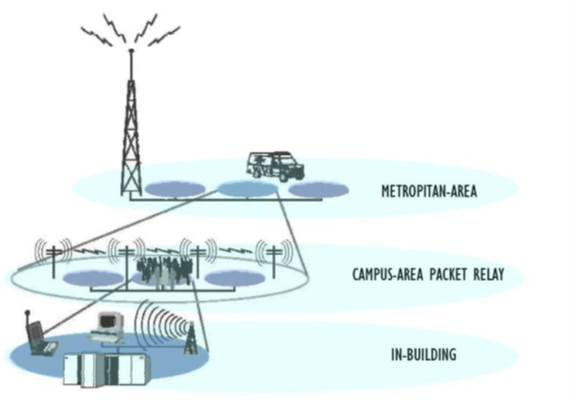
\includegraphics[width=0.85\textwidth]{img/inquinamento-elettromagnetico.png}
        \caption{\scriptsize Inquinamento EMI}
        \end{figure}
    \end{columns}
\end{frame}

\section{Architetture}

% Architetture proposte
\begin{frame}{Architetture Amplificatori: OTA Miller vs OTA Nauta}
    \begin{columns}
        \column{0.5\textwidth}
        \begin{block}{OTA Miller (tradizionale)}
            \begin{itemize}
                \item Coppia differenziale e specchi
                \item Complessità strutturale
                \item Nodi interni vulnerabili
                \item Asimmetria dello slew rate
            \end{itemize}
        \end{block}
        
        \vspace{0.2cm}
        \begin{figure}
            \centering
            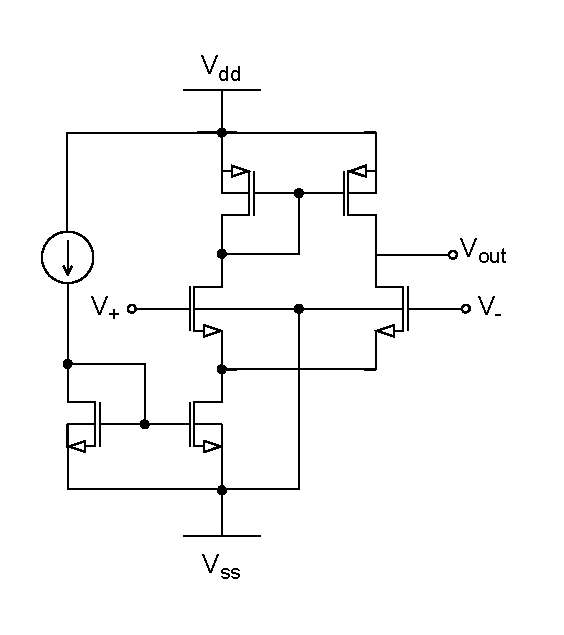
\includegraphics[width=0.75\textwidth]{img/sch/miller.drawio.pdf}
            \caption{\scriptsize Schema OTA Miller}
        \end{figure}
        
        \column{0.5\textwidth}
        \begin{block}{OTA Nauta (inverter-based)}
            \begin{itemize}
                \item Basato su inverter CMOS
                \item Semplice, senza nodi interni
                \item Simmetria intrinseca
                \item Potenzialmente più immune
            \end{itemize}
        \end{block}
        
        \vspace{0.2cm}
        \begin{figure}
            \centering
            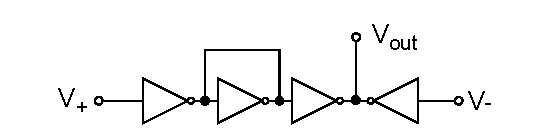
\includegraphics[width=0.75\textwidth]{img/sch/basic_nauta.pdf}
            \caption{\scriptsize Schema OTA Nauta}   
        \end{figure}
    \end{columns}
\end{frame}

\section{Obiettivi e Metodologia}

% Obiettivi dello studio
\begin{frame}{Obiettivi dello Studio}
    \begin{columns}
        \column{0.58\textwidth}
        \begin{block}{Scopo della ricerca}
            \begin{itemize}
                \item Confrontare l'immunità EMI dell'architettura Nauta vs Miller
                \item Verificare vantaggi degli amplificatori basati su inverter
                \item Analizzare influenza della tensione di alimentazione
                \item Valutare l'effetto della capacità di carico
            \end{itemize}
        \end{block}
        
        \begin{alertblock}{Ipotesi di partenza}
            L'architettura Nauta, grazie alla sua semplicità e simmetria, dovrebbe mostrare una migliore immunità alle EMI rispetto all'architettura Miller.
        \end{alertblock}
        
        \column{0.38\textwidth}
        \begin{block}{Varianti analizzate}
            \begin{itemize}\small
                \item \textbf{Architetture:} 
                      \begin{itemize}\footnotesize
                          \item Singolo stadio
                          \item Doppio stadio
                      \end{itemize}
                \item \textbf{Tensioni:} 
                      \begin{itemize}\footnotesize
                          \item 0.5V (solo Nauta)
                          \item 1V
                          \item 1.8V
                      \end{itemize}
                \item \textbf{Capacità:} 
                      \begin{itemize}\footnotesize
                          \item 1pF
                          \item 10pF
                      \end{itemize}
            \end{itemize}
        \end{block}
    \end{columns}
\end{frame}

% Metodologia di simulazione
\begin{frame}{Metodologia di Simulazione}
    \begin{columns}
        \column{0.4\textwidth}
        \begin{block}{Configurazione voltage follower}
            \begin{itemize}\small
                \item \textbf{Caso peggiore per le EMI:} 
                      \begin{itemize}\footnotesize
                          \item Retroazione amplifica gli effetti
                          \item Evidenzia piccole vulnerabilità
                      \end{itemize}
                \item EMI: segnali sinusoidali (1 MHz - 4 GHz)
                \item Misurazione dell'offset DC indotto
                \item Studio in diverse configurazioni
            \end{itemize}
        \end{block}
        
        \begin{block}{Parametri target}
            \begin{itemize}\small
                \item Guadagno: $\approx$ 40 dB
                \item Margine di fase: $\geq$ 60°
                \item Regione: saturazione
            \end{itemize}
        \end{block}
        
        \column{0.6\textwidth}
        \begin{figure}
            \centering
            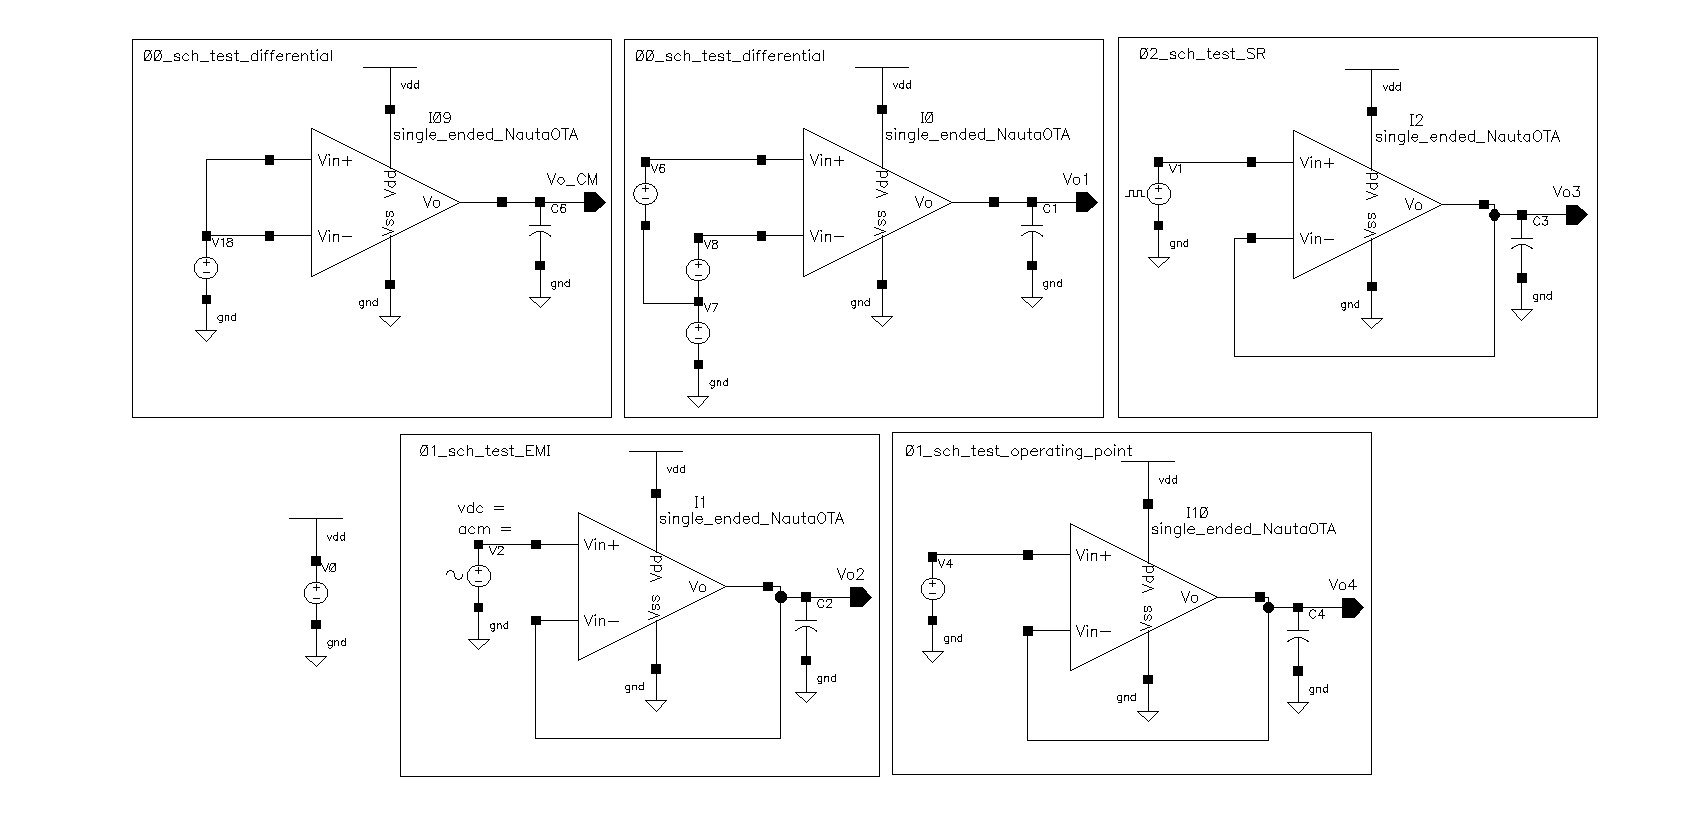
\includegraphics[width=\textwidth]{img/nauta/single/sim_nauta_single_stage.png}
            \caption{Setup test EMI}
        \end{figure}
    \end{columns}
\end{frame}

\section{Risultati}

% Risultati Nauta singolo stadio
\begin{frame}{Risultati: OTA Nauta a Stadio Singolo}
    \begin{columns}
        \column{0.48\textwidth}
        \begin{figure}
            \centering
            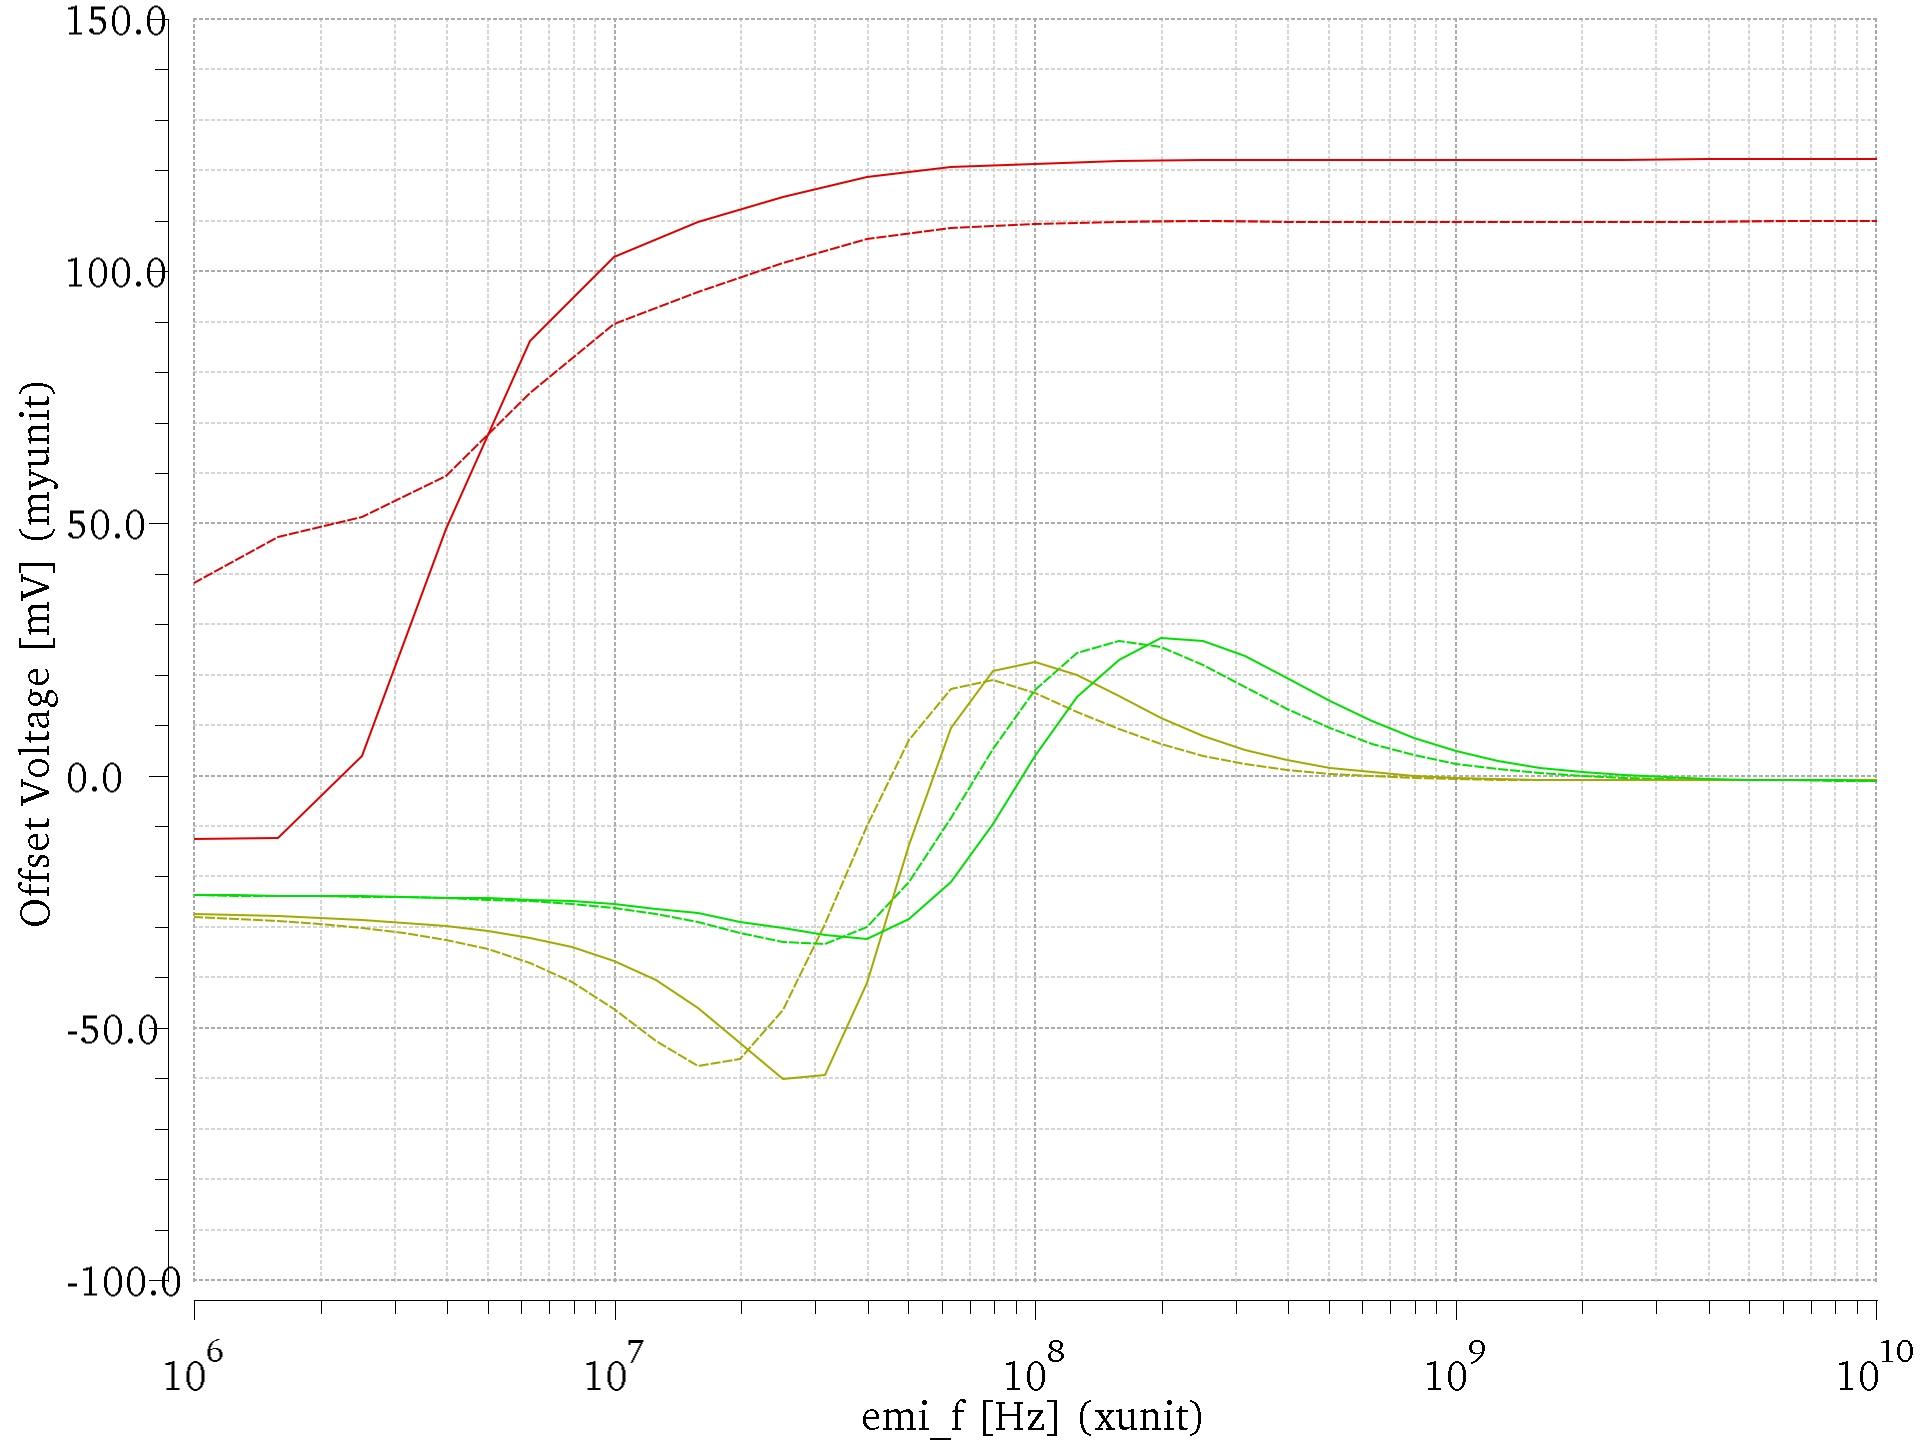
\includegraphics[width=\textwidth]{img/nauta/single/emi_comparison.jpg}
            \caption{\scriptsize EMI rejection Nauta}
        \end{figure}
        
        \footnotesize
        \begin{table}
        \begin{tabular}{@{}lccc@{}}
            \toprule
            \textbf{V} & \textbf{PM} & \textbf{GBW} & \textbf{SR} \\
            \midrule
            0.5V & 72° & 352 kHz & 3.1 V/$\mu$s \\
            1V & 78° & 50 MHz & 19 V/$\mu$s \\
            1.8V & 79° & 235 MHz & 67 V/$\mu$s \\
            \bottomrule
        \end{tabular}
        \caption{\scriptsize Parametri a varie tensioni}
        \end{table}
        \column{0.48\textwidth}
        \begin{block}{Osservazioni chiave}
            \begin{itemize}\small
                \item Immunità EMI eccellente per V$_{alim}$ = 1V e 1.8V
                \item Offset max: < 15mV (1V, 1.8V)
                \item Simmetria dello slew rate
                \item Ottime prestazioni alte frequenze
            \end{itemize}
        \end{block}
        
        \begin{alertblock}{Effetto capacità di carico (1pF→10pF)}
            \begin{itemize}\small
                \item Riduzione GBW (50→5 MHz)
                \item Riduzione SR (19→11 V/$\mu$s)
                \item Minimo impatto su immunità EMI
            \end{itemize}
        \end{alertblock}
    \end{columns}
\end{frame}

% Risultati Miller singolo stadio
\begin{frame}{Risultati: OTA Miller a Stadio Singolo}
    \begin{columns}
        \column{0.48\textwidth}
        \begin{figure}
            \centering
            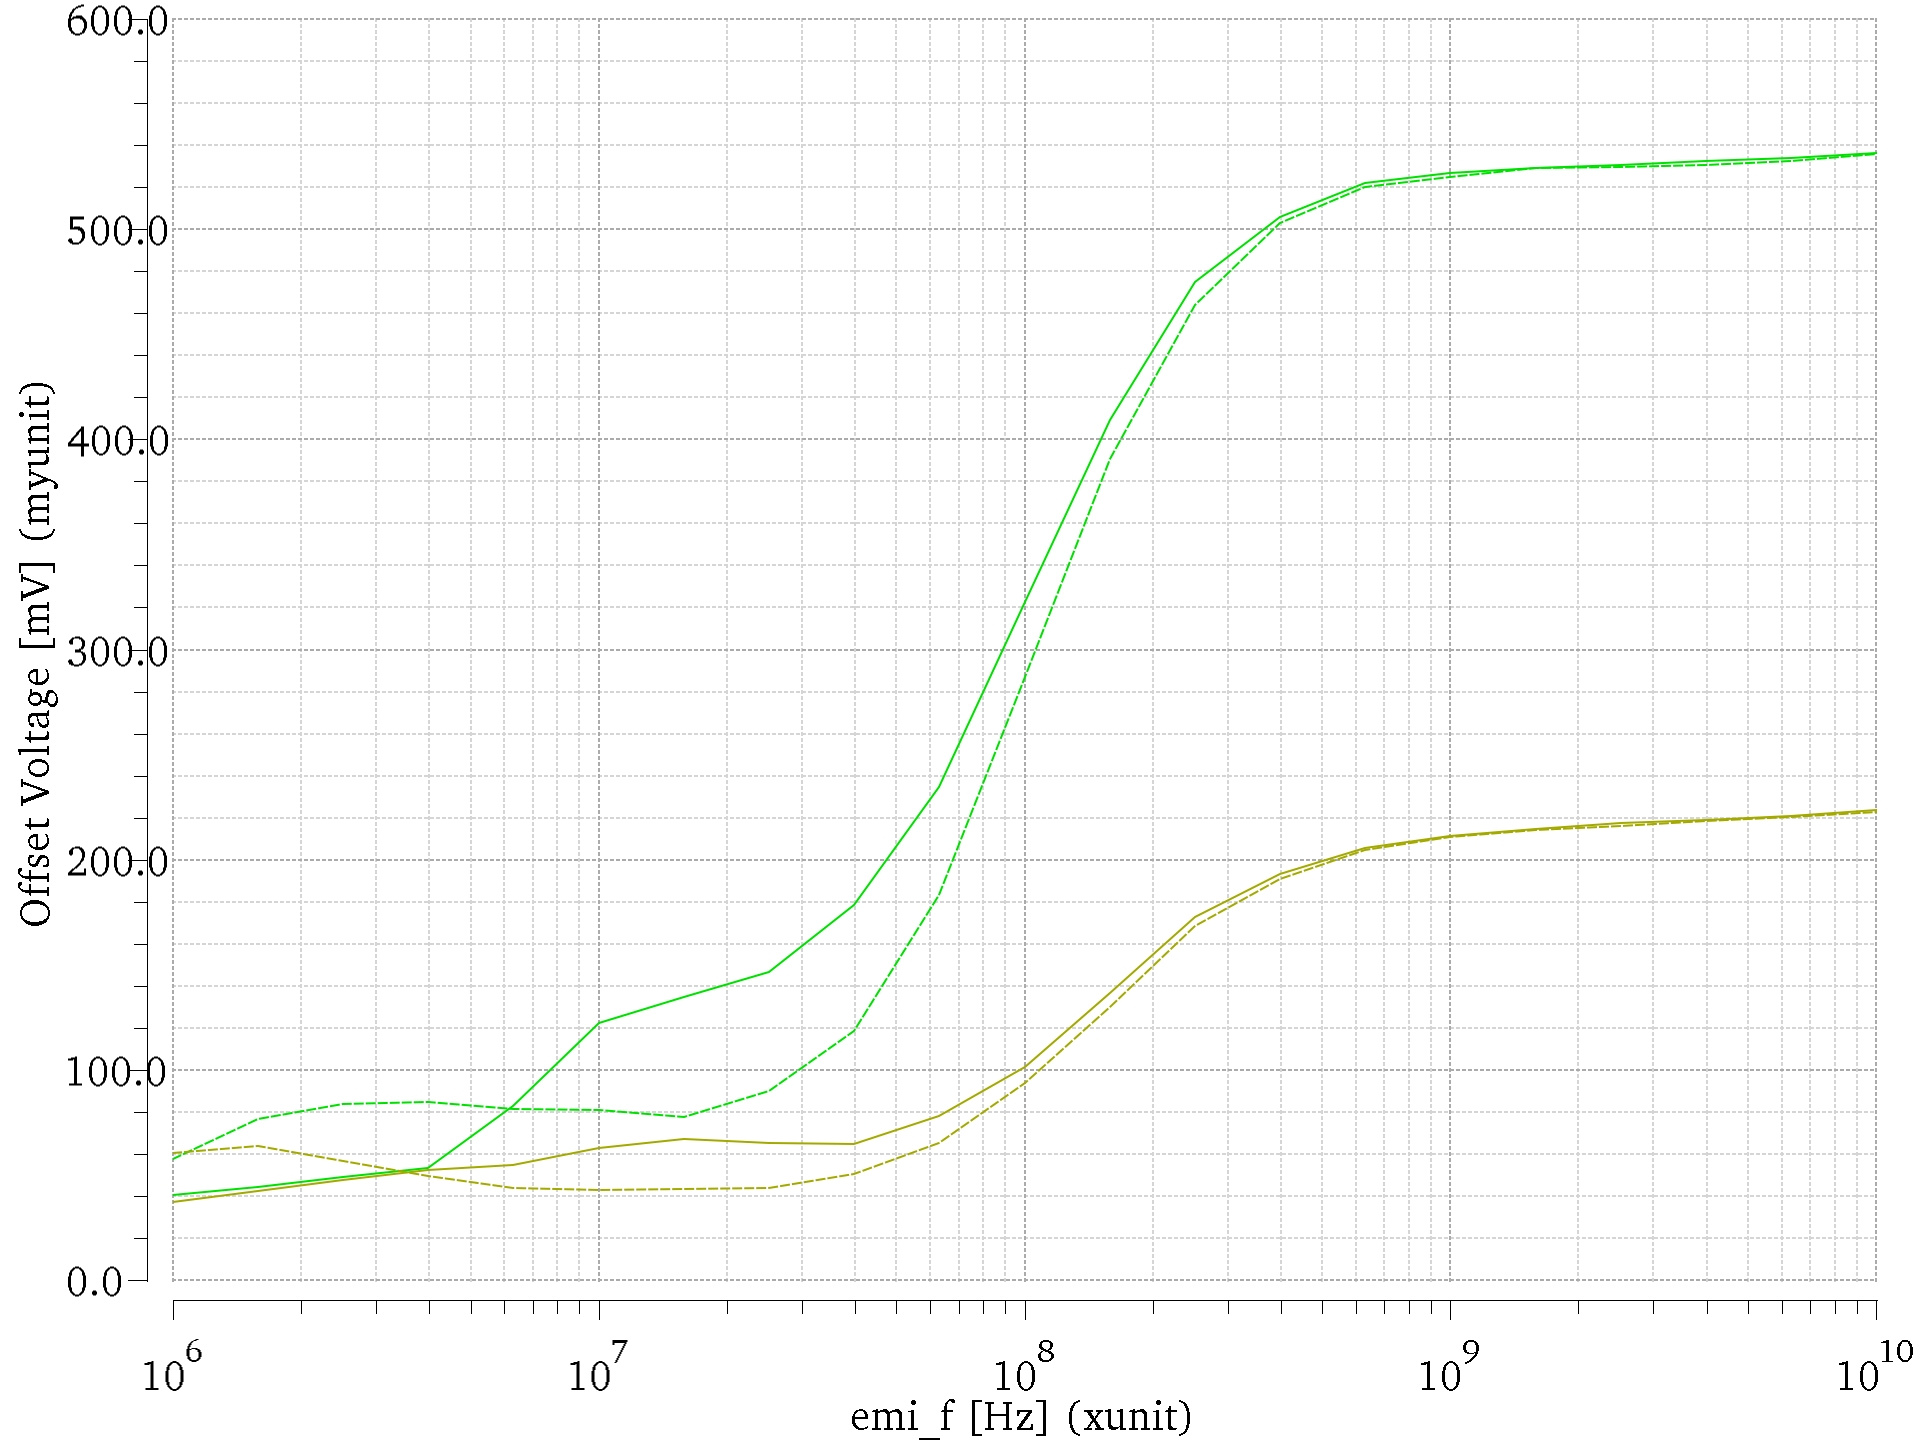
\includegraphics[width=\textwidth]{img/miller/single/emi_comparison.jpg}
            \caption{\scriptsize EMI rejection Miller}
        \end{figure}
        
        \footnotesize
        \begin{table}[h]
        \begin{tabular}{@{}lccc@{}}
            \toprule
            \textbf{C$_L$} & \textbf{PM} & \textbf{GBW} & \textbf{SR} \\
            \midrule
            1 pF & 78° & 26 MHz & 17 V/$\mu$s \\
            10 pF & 89° & 3 MHz & 2 V/$\mu$s \\
            \bottomrule
        \end{tabular}
        \caption{\scriptsize Effetto capacità di carico}
        \end{table}
        \column{0.48\textwidth}
        \begin{block}{Osservazioni chiave}
            \begin{itemize}\small
                \item Immunità EMI inferiore vs Nauta
                \item Offset max: > 50mV 
                \item Alta sensibilità 10-100 MHz
                \item Stabilità ridotta con C$_L$ = 10pF
            \end{itemize}
        \end{block}
        
        \begin{alertblock}{Limiti dell'architettura Miller}
            \begin{itemize}\small
                \item Coppia differenziale sensibile alle EMI
                \item Specchi di corrente creano asimmetrie
                \item Nodi interni facilitano accoppiamento EMI
                \item Maggiore sensibilità alla capacità di carico
            \end{itemize}
        \end{alertblock}
    \end{columns}
\end{frame}

% Risultati Nauta doppio stadio
\begin{frame}{Risultati: OTA Nauta a Doppio Stadio}
    \begin{columns}
        \column{0.48\textwidth}
        \begin{figure}
            \centering
            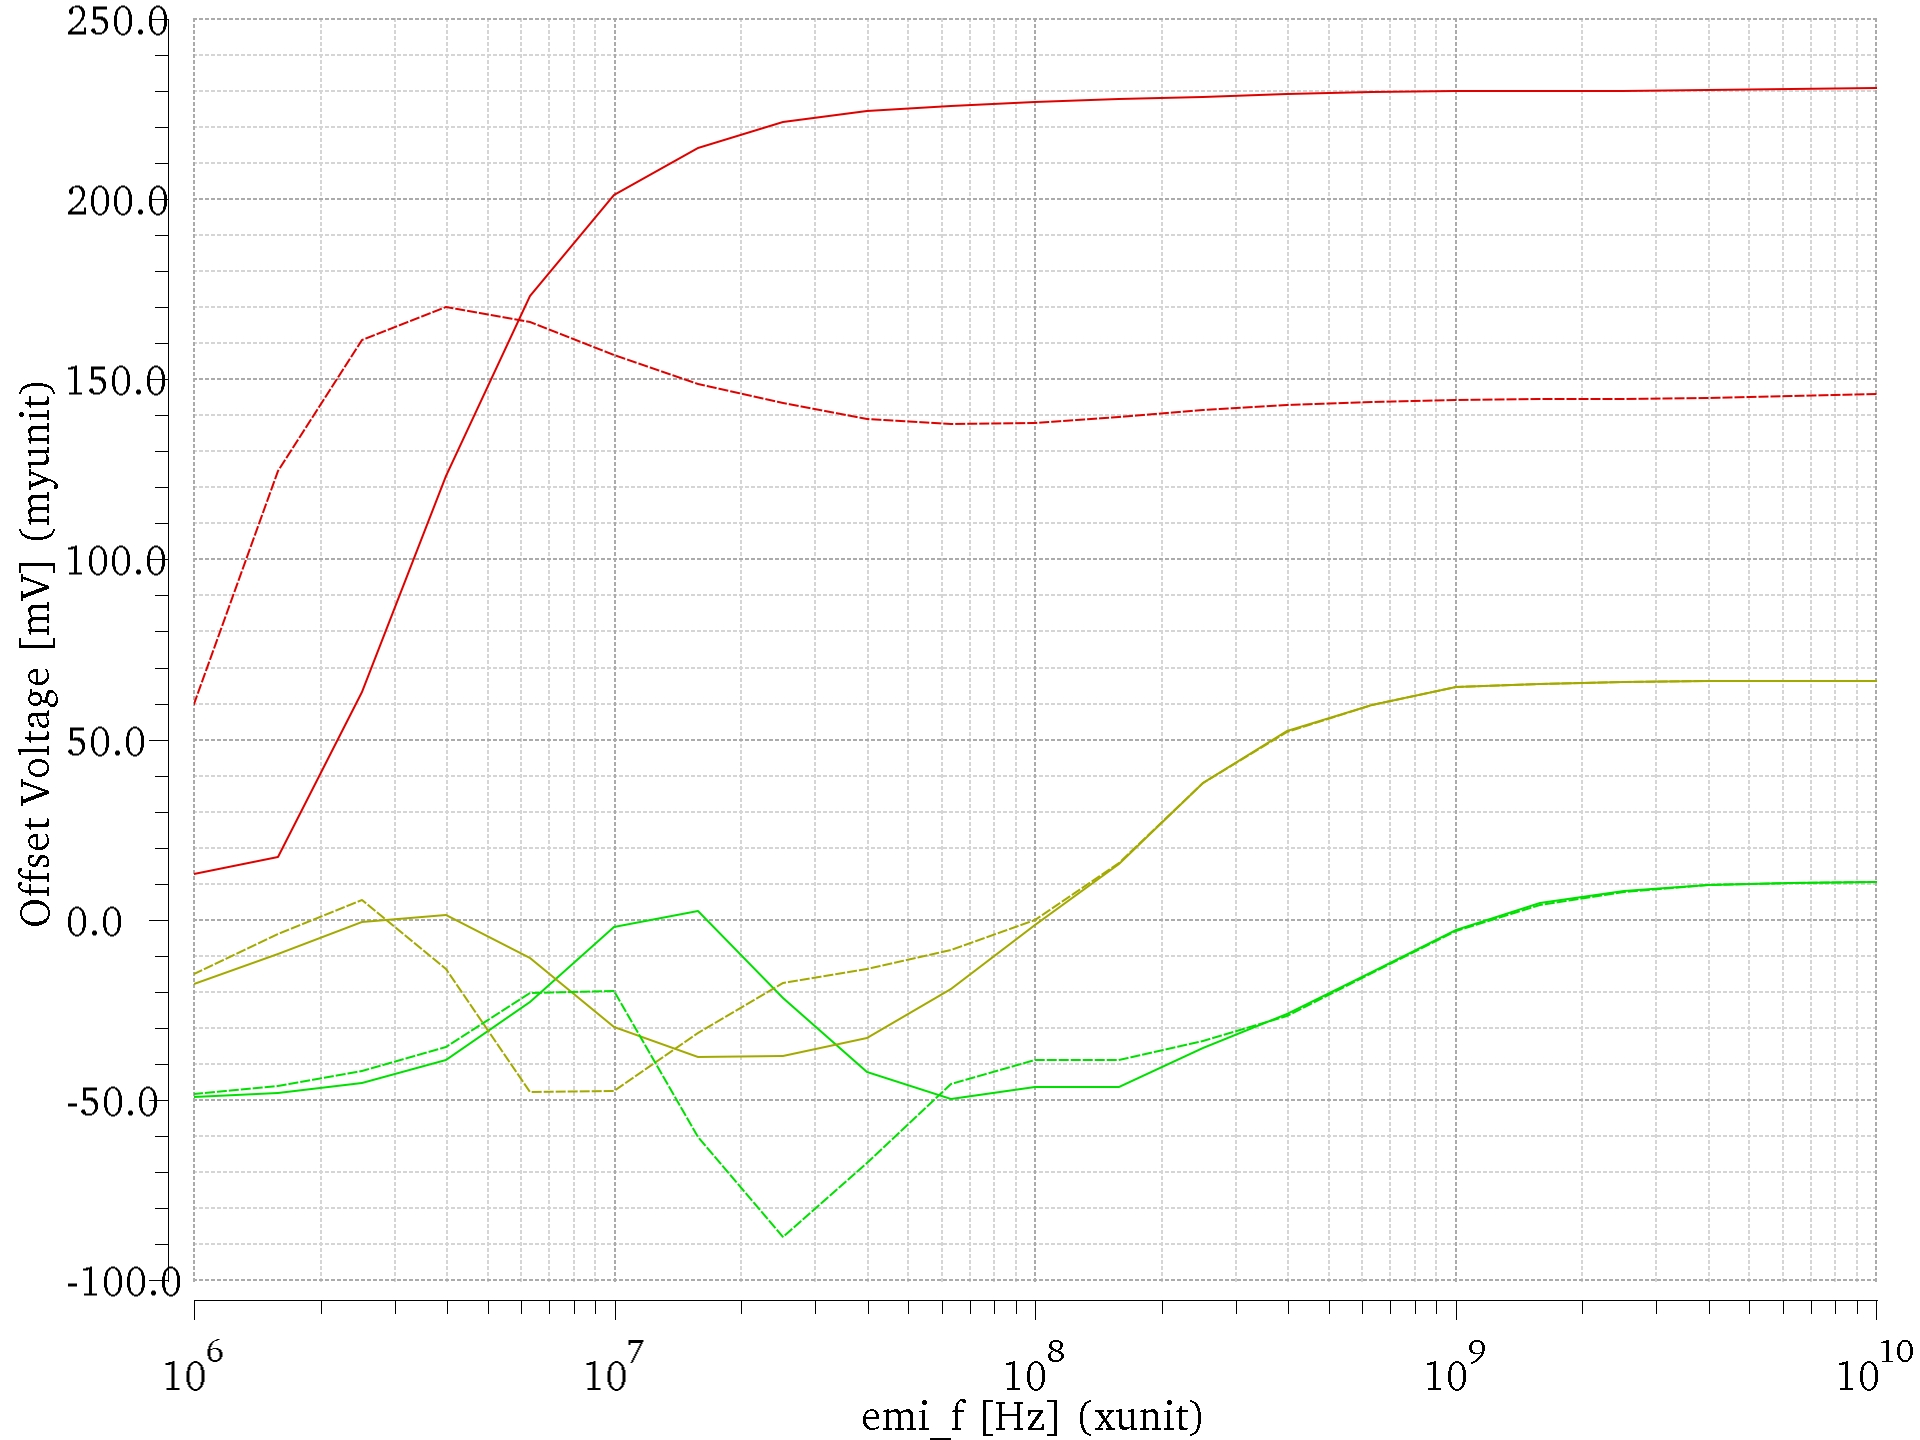
\includegraphics[width=\textwidth]{img/nauta/double/emi_comparison.jpg}
            \caption{\scriptsize EMI rejection Nauta (2 stadi)}
        \end{figure}
        
        \scriptsize
        \begin{table}
            \begin{tabular}{@{}lccc@{}}
                \toprule
                \textbf{V} & \textbf{PM} & \textbf{GBW} & \textbf{Gain} \\
                \midrule
                0.5V & 59° & 85 kHz & 73 dB \\
                1V & 68° & 11 MHz & 80 dB \\
                1.8V & 63° & 123 MHz & 76 dB \\
                \bottomrule
            \end{tabular}
            \caption{\scriptsize Parametri a varie tensioni}
        \end{table}
        \column{0.48\textwidth}
        \begin{block}{Osservazioni chiave}
            \begin{itemize}\small
                \item Guadagno elevato (>70 dB)
                \item Sensibilità EMI > stadio singolo
                \item Maggiore influenza tensione
                \item Maggiore dipendenza dal carico
                \item Alte performance a 1.8V
            \end{itemize}
        \end{block}
        
        \begin{alertblock}{Effetto capacità di carico (1pF→10pF)}
            \begin{itemize}\small
                \item Riduzione significativa PM (68°→33°)
                \item GBW quasi invariato
                \item Maggiore impatto su immunità EMI
                \item Riduzione SR del 50\%
            \end{itemize}
        \end{alertblock}
    \end{columns}
\end{frame}

% Risultati Miller doppio stadio
\begin{frame}{Risultati: OTA Miller a Doppio Stadio}
    \begin{columns}
        \column{0.48\textwidth}
        \begin{figure}
            \centering
            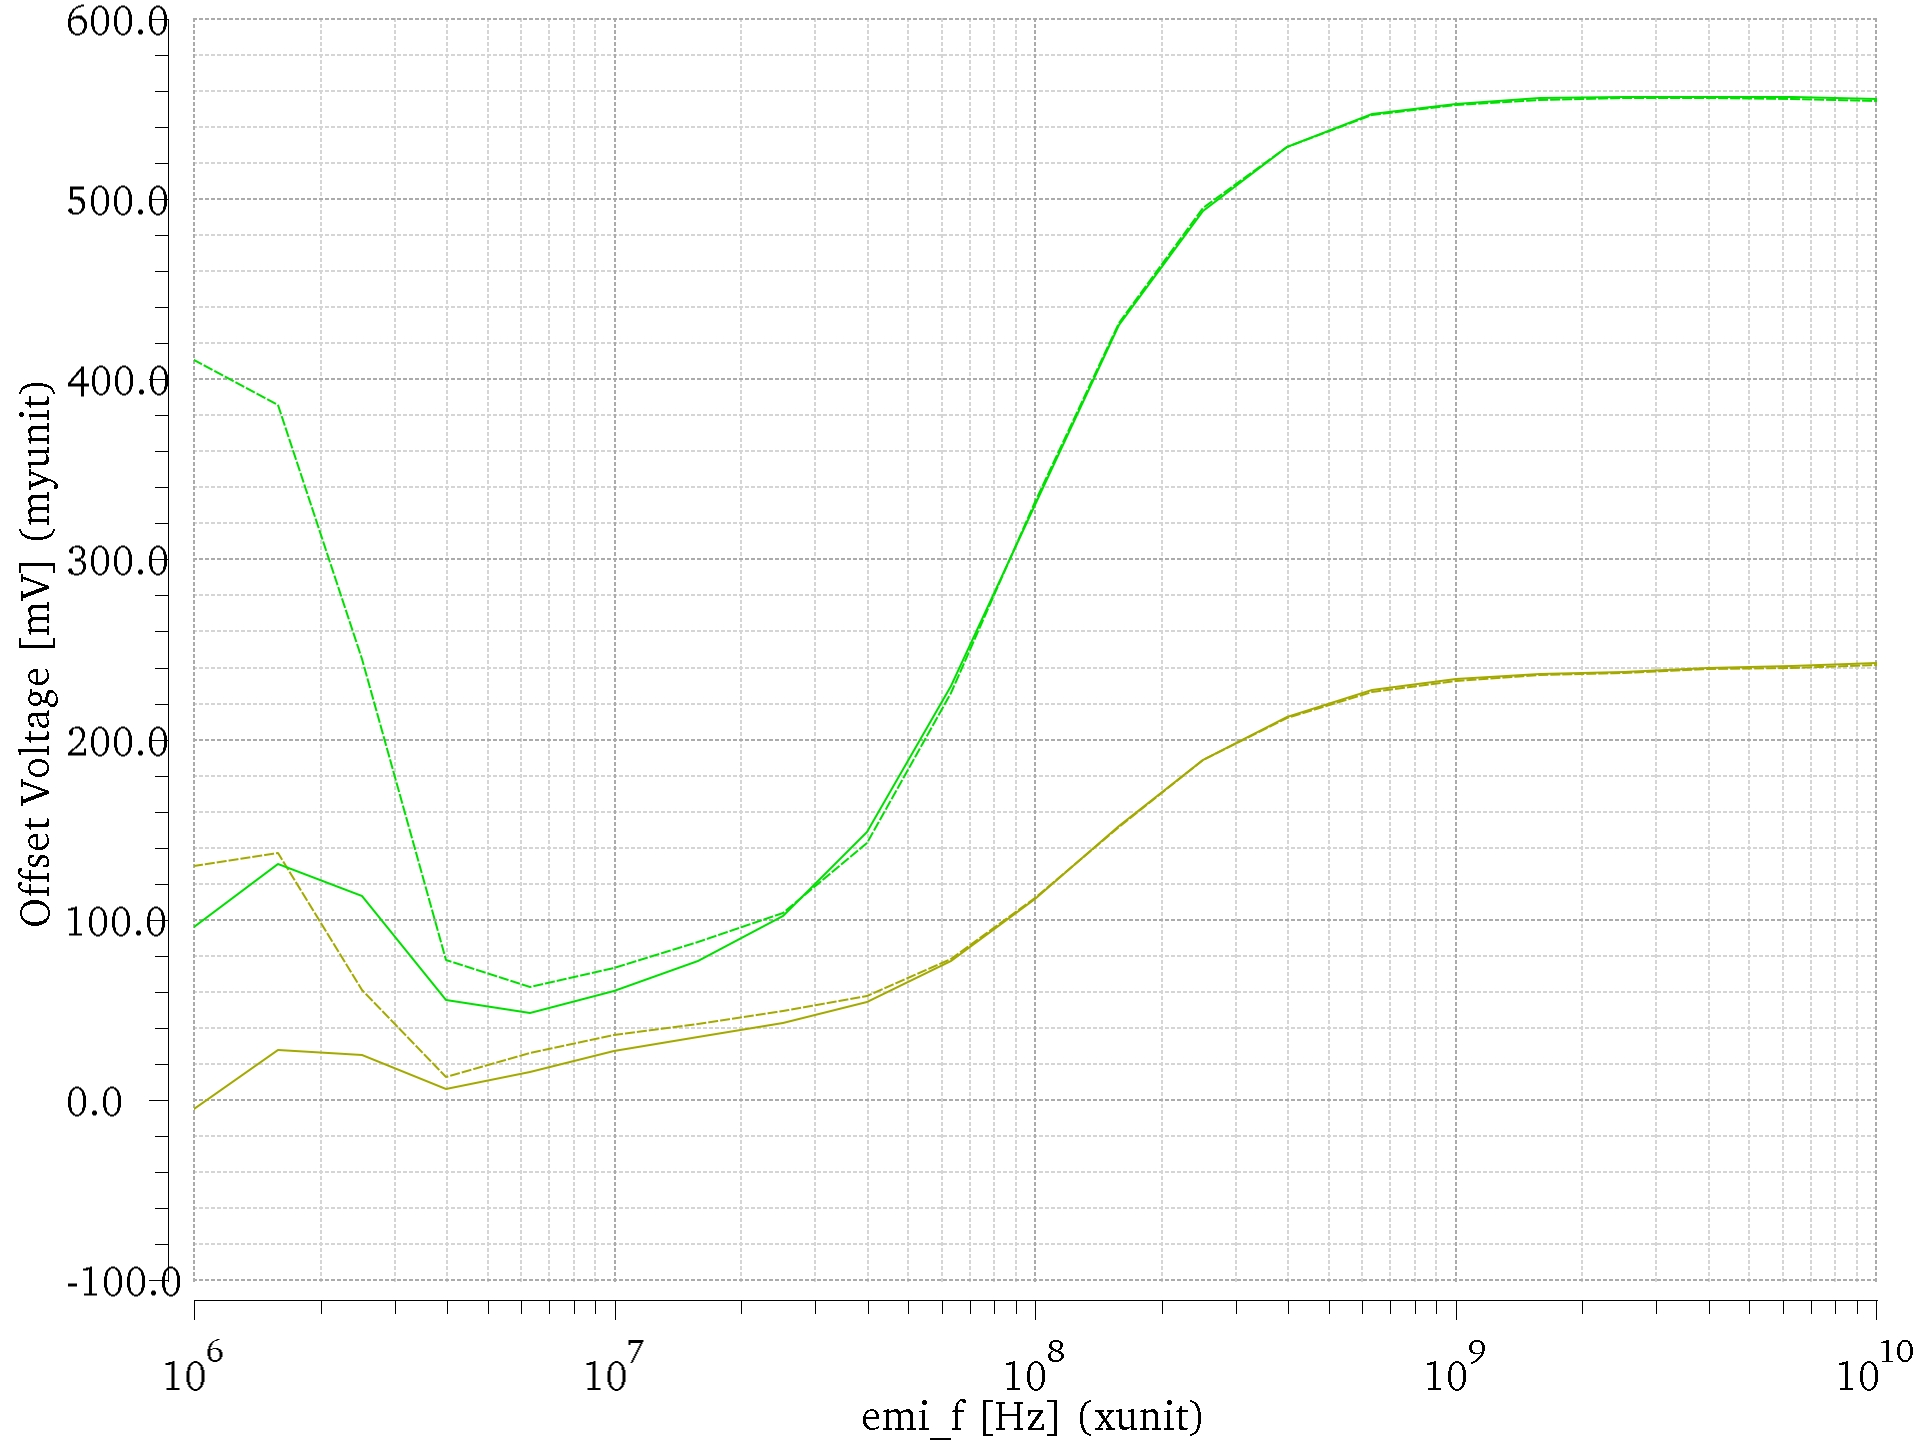
\includegraphics[width=\textwidth]{img/miller/double/emi_comparison.jpg}
            \caption{\scriptsize EMI rejection Miller (2 stadi)}
        \end{figure}
        
        \scriptsize
        \begin{table}
            \begin{tabular}{@{}lccc@{}}
                \toprule
                \textbf{Param} & \textbf{1pF} & \textbf{10pF} & \textbf{Unità} \\
                \midrule
                Gain & 76 dB & 76 dB & dB \\
                PM & 62° & 78° & ° \\
                GBW & 16 MHz & 2 MHz & MHz \\
                \bottomrule
            \end{tabular}
            \caption{\scriptsize Effetto capacità di carico}
        \end{table}
        \column{0.48\textwidth}
        \begin{block}{Osservazioni chiave}
            \begin{itemize}\small
                \item Guadagno comparabile con Nauta
                \item Suscettibilità EMI maggiore
                \item Offset indotto fino a 200mV
                \item Migliore stabilità con carichi elevati
            \end{itemize}
        \end{block}
        
        \begin{alertblock}{Confronto con Nauta doppio stadio}
            \begin{itemize}\small
                \item Performance generali inferiori
                \item GBW e SR maggiori per Nauta
                \item Maggiore sensibilità alle EMI
                \item Minor dipendenza dai parametri di processo
            \end{itemize}
        \end{alertblock}
    \end{columns}
\end{frame}

% Confronto frequenze
\begin{frame}{Analisi per Bande di Frequenza}
    \begin{columns}
        \column{0.45\textwidth}
        \begin{figure}
            \centering
            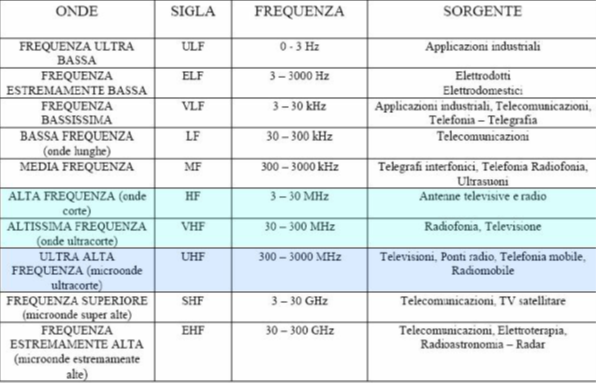
\includegraphics[width=\textwidth]{img/suddivizione-onde.png}
            \caption{\scriptsize Risposta a diverse frequenze EMI}
        \end{figure}
        
        \column{0.51\textwidth}
        \begin{block}{Comportamento in frequenza}
            \begin{itemize}\small
                \item \textbf{Basse frequenze (1-10 MHz):}
                      \begin{itemize}\footnotesize
                          \item Entrambe le architetture sensibili
                          \item Vantaggio Nauta meno marcato
                      \end{itemize}
                \item \textbf{Medie frequenze (10-100 MHz):}
                      \begin{itemize}\footnotesize
                          \item Picco di sensibilità per Miller
                          \item Nauta mantiene immunità elevata
                      \end{itemize}
                \item \textbf{Alte frequenze (>100 MHz):}
                      \begin{itemize}\footnotesize
                          \item Differenza drastica tra architetture
                          \item Immunità Nauta fino a 10x superiore
                      \end{itemize}
            \end{itemize}
        \end{block}
    \end{columns}
\end{frame}

% Confronto complessivo
\begin{frame}{Confronto EMI tra Architetture Nauta e Miller}
    \begin{columns}
        \column{0.48\textwidth}
        \begin{figure}
            \centering
            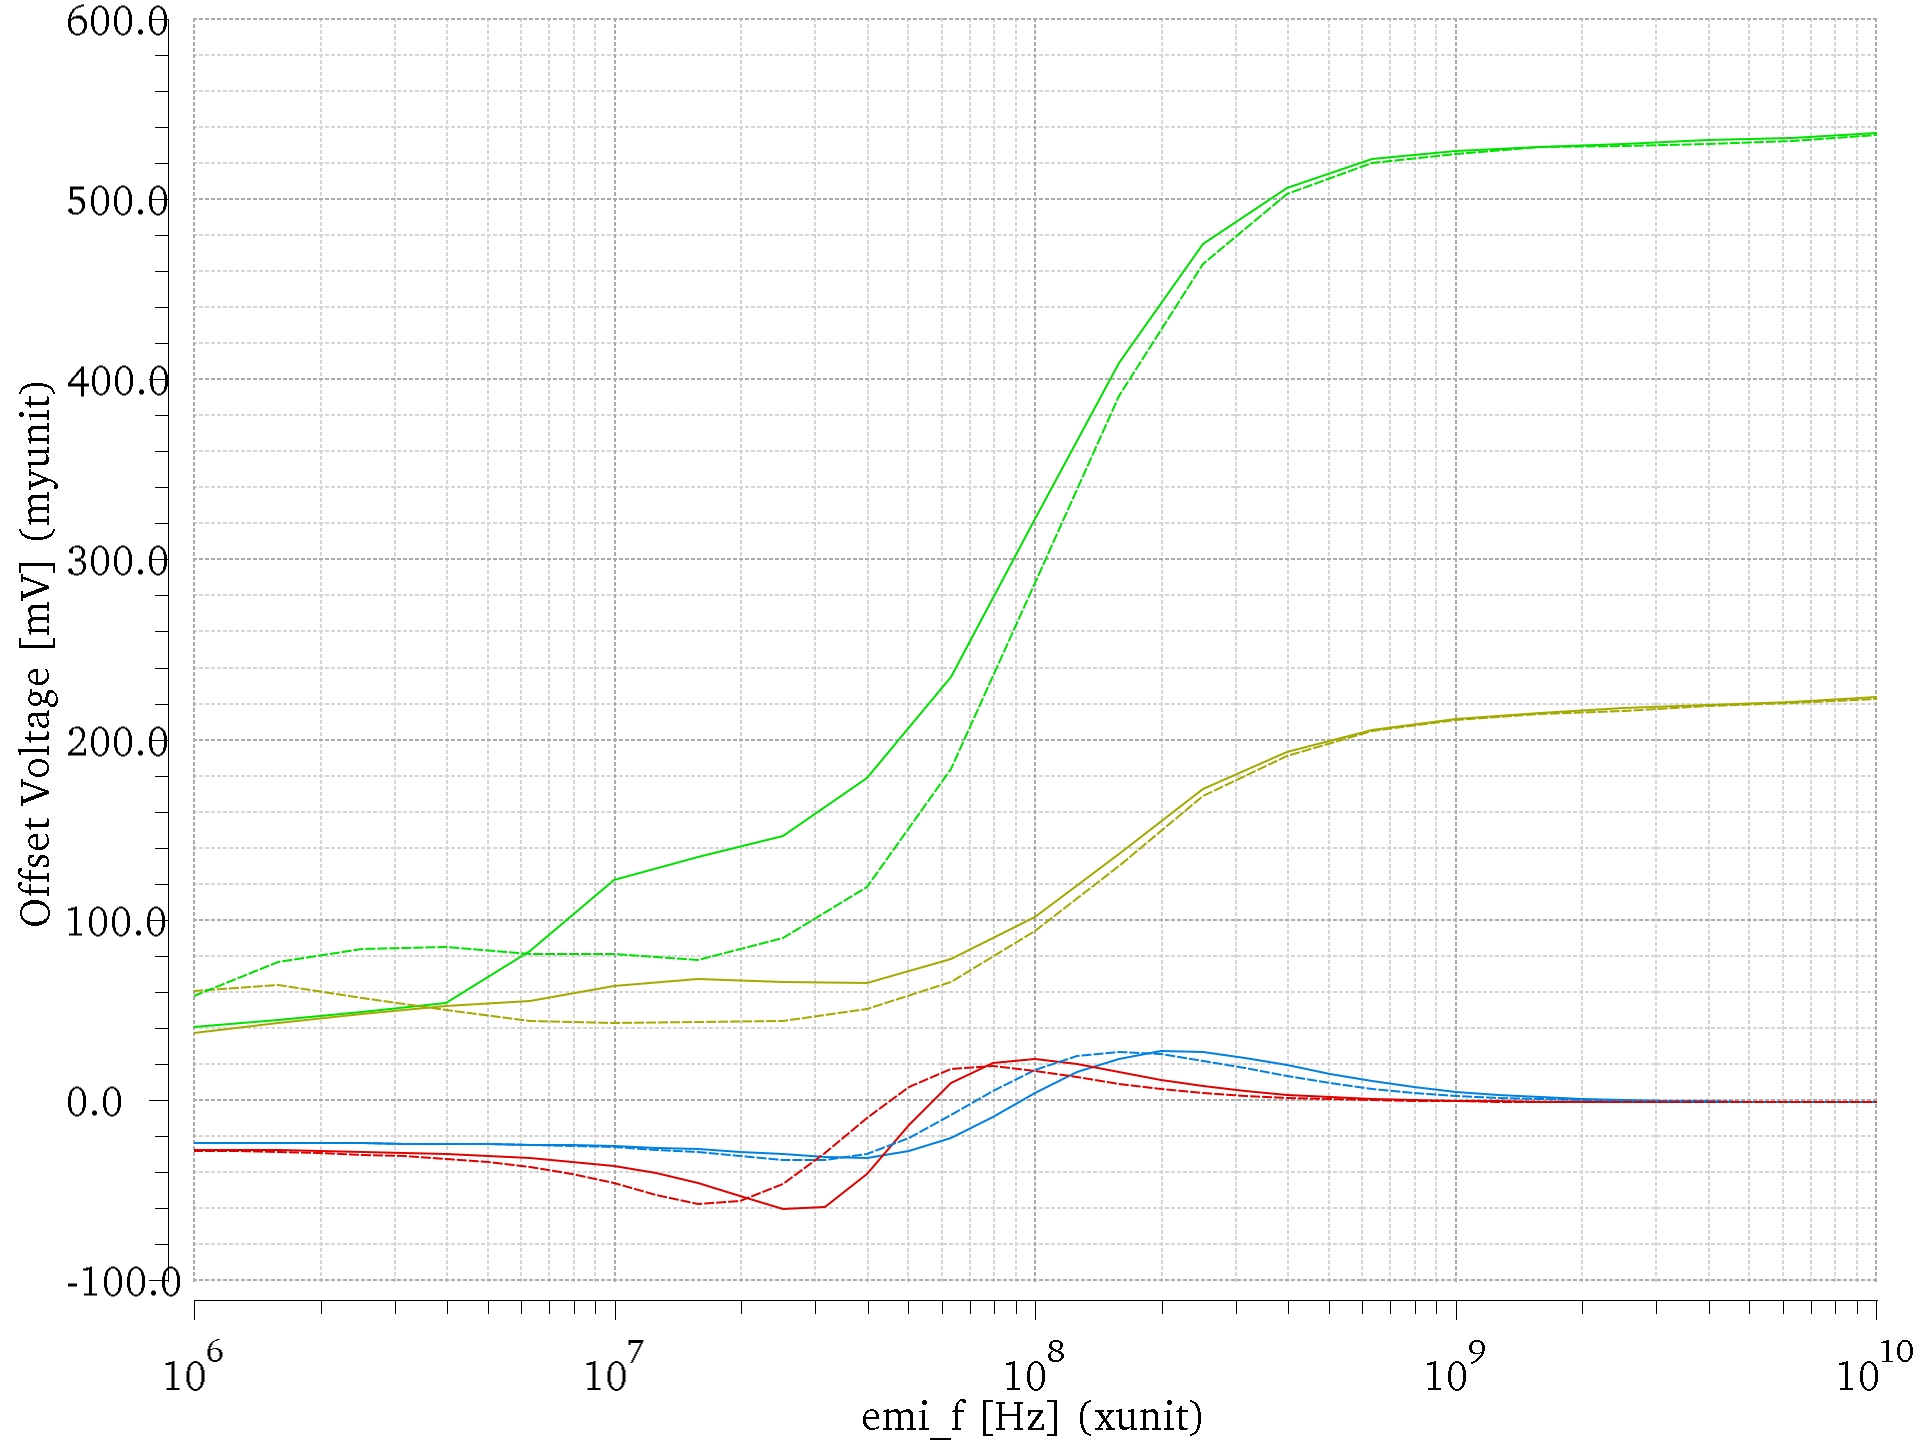
\includegraphics[width=\textwidth]{img/emi/emi_comparison_miller_nauta_single_stage.jpg}
            \caption{\scriptsize Confronto stadio singolo}
        \end{figure}
        
        \column{0.48\textwidth}
        \begin{figure}
            \centering
            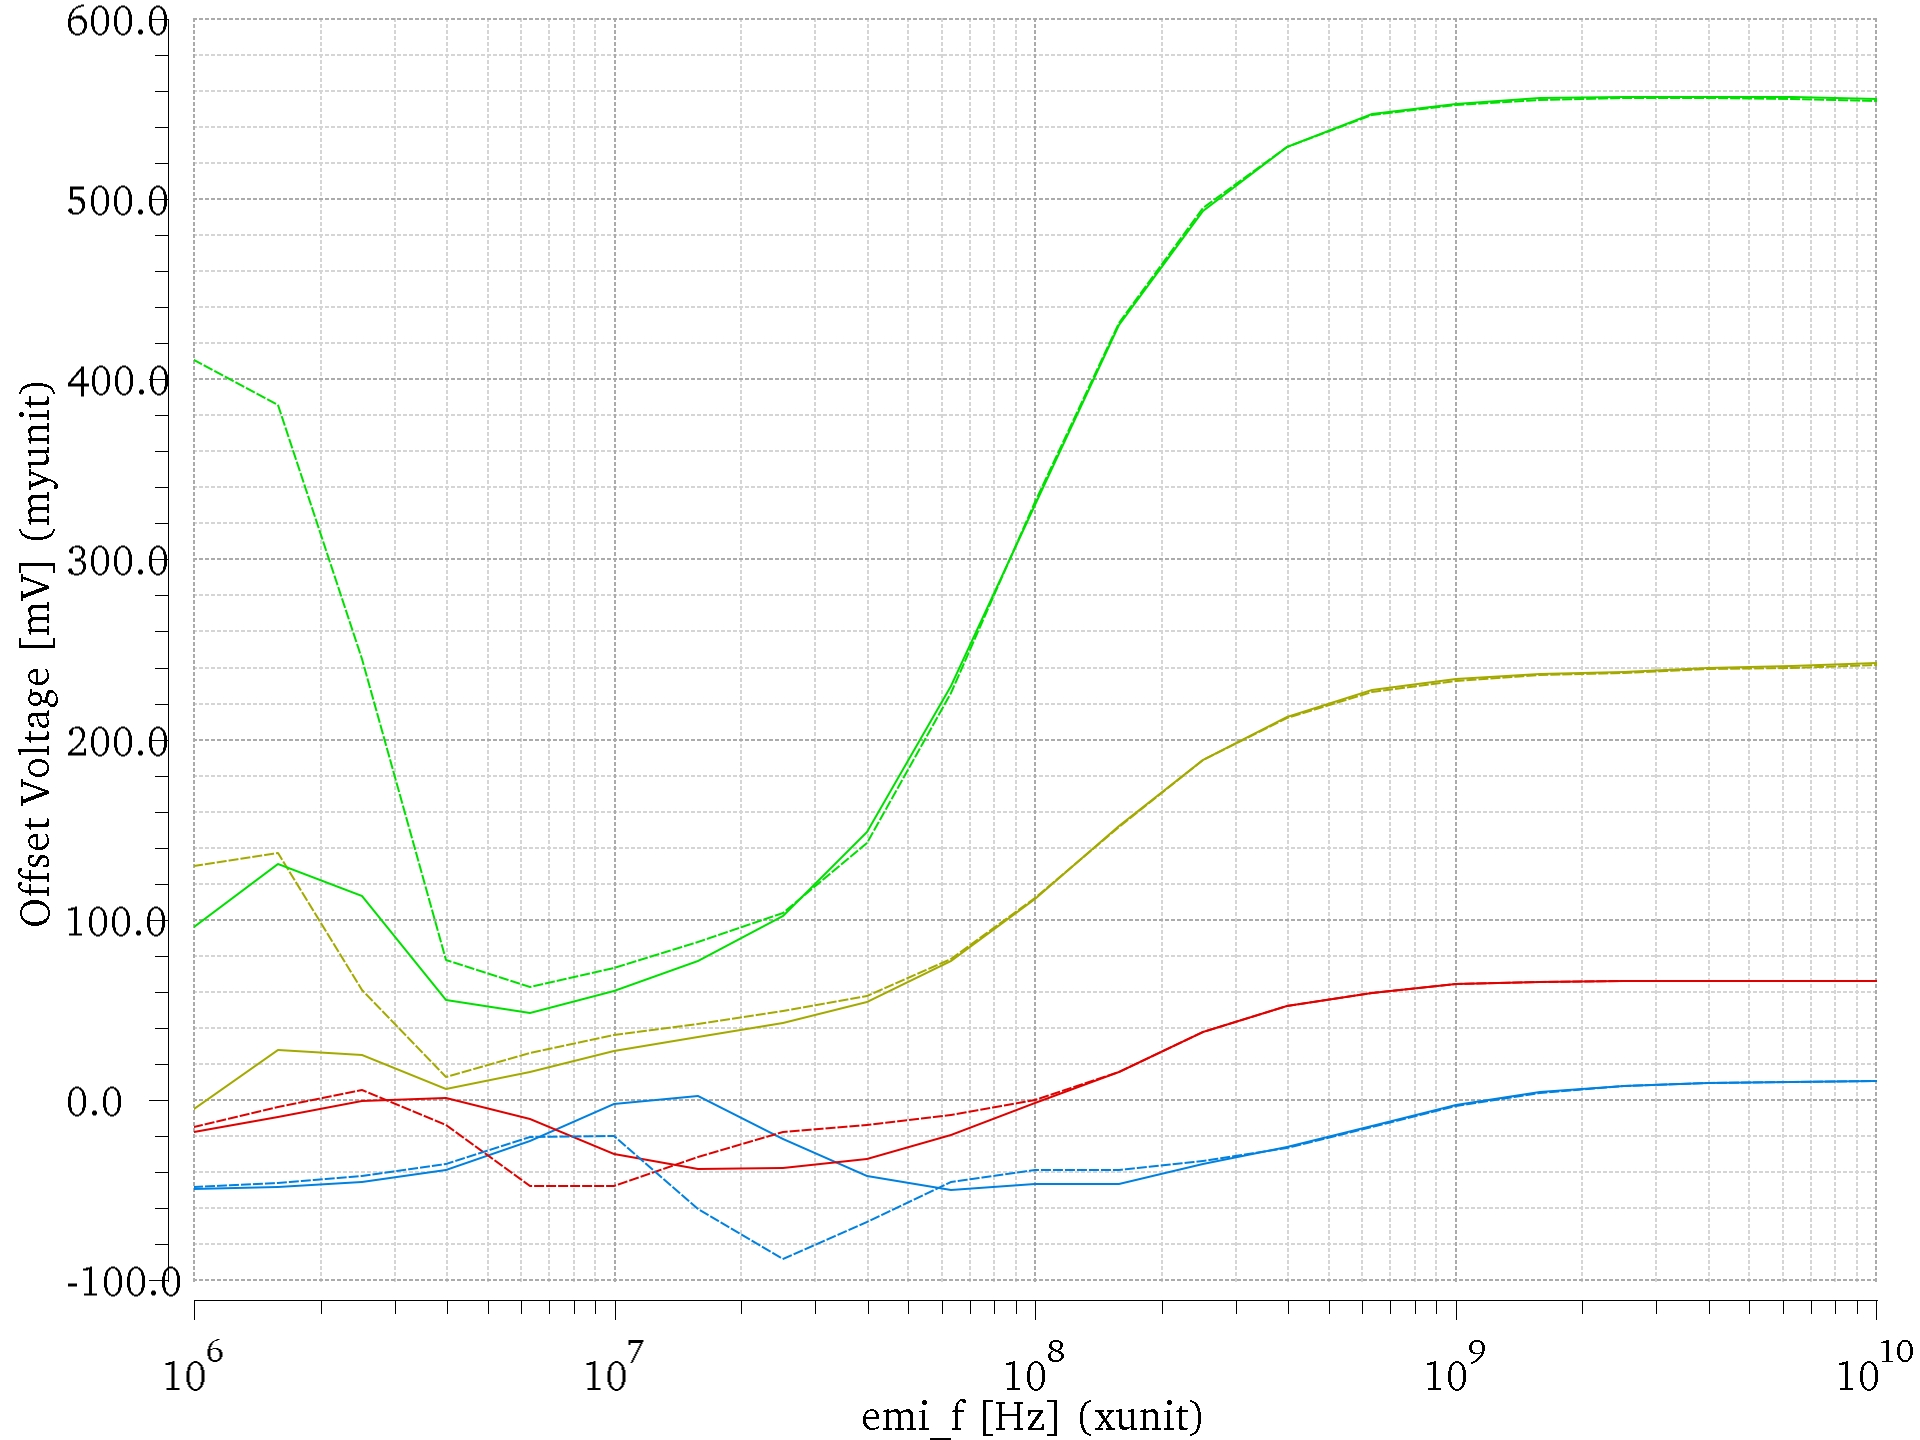
\includegraphics[width=\textwidth]{img/emi/emi_comparison_miller_nauta_two_staged.jpg}
            \caption{\scriptsize Confronto doppio stadio}
        \end{figure}
    \end{columns}
    
    \vspace{0.2cm}
    \begin{block}{Risultati chiave}
        \begin{itemize}\small
            \item OTA Nauta: immunità EMI nettamente superiore in tutte le configurazioni
            \item Prestazioni eccellenti ad alte frequenze (>1 GHz) per Nauta
            \item Maggiore dipendenza dalla tensione nell'OTA Nauta
            \item Suscettibilità EMI aumenta nelle configurazioni a doppio stadio
            \item Offset indotto in Nauta fino a un ordine di grandezza inferiore rispetto a Miller
        \end{itemize}
    \end{block}
\end{frame}

\section{Conclusioni}

% Studio parametrico
\begin{frame}{Studio Parametrico dell'Immunità EMI}
    \begin{columns}
        \column{0.48\textwidth}
        \begin{block}{Effetto della tensione di alimentazione}
            \begin{itemize}\small
                \item Migliore immunità con tensioni più elevate
                \item Nauta: immunità cresce con V$_{alim}$
                \item Miller: meno dipendente da V$_{alim}$
                \item Rapporto ottimale a 1.8V
            \end{itemize}
        \end{block}
        
        \begin{block}{Effetto del numero di stadi}
            \begin{itemize}\small
                \item Singolo stadio sempre più immune
                \item Cascata di stadi riduce l'immunità
                \item Aumento della complessità circuitale
                \item Trade-off tra guadagno e immunità EMI
            \end{itemize}
        \end{block}
        
        \column{0.48\textwidth}
        \begin{block}{Effetto della capacità di carico}
            \begin{itemize}\small
                \item Nauta: minore dipendenza dal carico
                \item Miller: riduzione drastica di performance
                \item Impatto limitato sull'immunità EMI
                \item Maggior effetto su GBW e SR
            \end{itemize}
        \end{block}
        
        \begin{alertblock}{Cause dell'immunità EMI di Nauta}
            \begin{itemize}\small
                \item Simmetria intrinseca della topologia
                \item Assenza di nodi vulnerabili
                \item Bilanciamento percorsi NMOS e PMOS
                \item Semplicità circuitale complessiva
                \item Minore impedenza dei nodi interni
            \end{itemize}
        \end{alertblock}
    \end{columns}
\end{frame}

% Conclusioni
\begin{frame}{Conclusioni}
    \begin{block}{Risultati principali}
        \begin{itemize}\small
            \item Architettura Nauta: suscettibilità EMI significativamente inferiore
            \item Immunità EMI migliora all'aumentare della tensione di alimentazione
            \item Singolo stadio più immune del doppio stadio
            \item Capacità di carico: impatto limitato sull'immunità EMI
            \item Simmetria degli inverter contribuisce alla robustezza EMI
        \end{itemize}
    \end{block}
    
    \vspace{0.2cm}
    \begin{alertblock}{Applicazioni}
        Nauta è efficace per amplificatori con elevata immunità EMI:
        \begin{itemize}\small
            \item Applicazioni a bassa tensione
            \item Ambienti EMI ostili (automotive, industriale)
            \item Sistemi portatili vicino a sorgenti EMI
        \end{itemize}
    \end{alertblock}
    
    \vspace{0.2cm}
    \begin{block}{Sviluppi futuri}
        \begin{itemize}\small
            \item Analisi post-layout
            \item Verifica sperimentale su chip prototipale
            \item Ottimizzazione per tensioni ultra-basse (<0.5V)
        \end{itemize}
    \end{block}
\end{frame}

% Bibliografia
\begin{frame}{Bibliografia}
    \setbeamertemplate{bibliography item}[article]
    \scriptsize
    \begin{thebibliography}{9}
        \bibitem{ref1} Richelli, A., Matig-a, G., Redouté, J.M. (2015). 
        \newblock{\emph{Design of a folded cascode opamp with increased immunity to conducted electromagnetic interference in 0.18 $\mu$m CMOS}}. 
        \newblock{Microelectronics Reliability, \textbf{55}(3-4), 654-661.}
        
        \bibitem{ref2} Rosa, A., Richelli, A., Colalongo, L. (2024). 
        \newblock{\emph{EMI Immunity of the Nauta Inverter-Based Amplifier}}. 
        \newblock{IEEE Int. Workshop on the EMC of Integrated Circuits, 15-18.}
        
        \bibitem{ref3} Nauta, B. (1992). 
        \newblock{\emph{A CMOS transconductance-C filter technique for very high frequencies}}. 
        \newblock{IEEE Journal of Solid-State Circuits, \textbf{27}(2), 142-153.}
        
        \bibitem{ref4} Richelli, A., Kennedy, S., Redouté, J.M. (2017). 
        \newblock{\emph{An EMI-Resistant Common-Mode Cancelation Differential Input Stage in UMC 180 nm CMOS}}. 
        \newblock{IEEE Trans. on EMC, \textbf{59}(6), 2049-2051.}
        
        \bibitem{ref5} Richelli, A. et al. (2016). 
        \newblock{\emph{Susceptibility of Operational Amplifiers to Conducted EMI Injected Through the Ground Plane into Their Output Terminal}}. 
        \newblock{IEEE Trans. on Reliability, \textbf{65}(3), 1369-1379.}
    \end{thebibliography}
\end{frame}

% Grazie per l'attenzione
\begin{frame}[plain]
    \begin{center}
        \vspace{1cm}
        {\color{unibs}\Huge Grazie per l'attenzione!}
        \vspace{1.2cm}
        
        
\includegraphics[height=1.8cm]{img/logo_unibs.pdf}
        
        \vspace{0.6cm}
        {\large \textit{Luca Brescia}}\\
        \vspace{0.2cm}
        {\footnotesize Università degli Studi di Brescia\\
        Dipartimento di Ingegneria dell'Informazione}
    \end{center}
\end{frame}

\end{document}